% PCCSL 507 Machine Learning Lab - Complete Record (joined, double-side print order)
% Order: Exp1=marks, Exp2=dataframe, Exp3=sales, Exp4=hours, Exp5=MLR, Exp6=SLR California
\documentclass[11pt,twoside]{article}

\usepackage[paper=letterpaper,top=0.7in,bottom=0.63in,left=0.75in,right=0.75in,headheight=24pt,headsep=0.14in,footskip=0.38in]{geometry}

\usepackage[T1]{fontenc}
\usepackage{mathptmx} % Times clone
\usepackage{xcolor}
\definecolor{primary}{HTML}{1F3864}
\definecolor{greytext}{HTML}{555555}
\definecolor{gridgrey}{HTML}{999999}
\usepackage{fancyhdr}
\usepackage{array}
\usepackage{colortbl}
\usepackage{parskip}
\setlength{\parindent}{0pt}
\setlength{\parskip}{4pt}
\setlength{\abovedisplayskip}{4pt}
\setlength{\belowdisplayskip}{4pt}
\setlength{\abovedisplayshortskip}{2pt}
\setlength{\belowdisplayshortskip}{2pt}
\usepackage{graphicx}
\usepackage{amsmath}
\usepackage{listings}
\lstset{basicstyle=\footnotesize\ttfamily, breaklines=true, frame=single, showstringspaces=false}

\pagestyle{fancy}
\fancyhf{}
\fancyhead[C]{\textcolor{primary}{\textbf{\small PCCSL 507 Machine Learning Laboratory Record}}}
\renewcommand{\headrulewidth}{0.75pt}
\renewcommand{\headrule}{\hbox to\headwidth{\color{primary}\leaders\hrule height \headrulewidth\hfill}}
\fancyfoot[C]{\footnotesize DEPARTMENT OF CSE \hfill CAPE COLLEGE OF ENGINEERING ALAPPUZHA \hfill Page No. \thepage}
\renewcommand{\footrulewidth}{0pt}

\newcommand{\expheading}[1]{{\fontsize{14}{17}\selectfont\textbf{#1}\par}}
\newcommand{\fullrule}{\noindent\rule{\textwidth}{0.6pt}\par}
% Break to next odd (right-side) page; inserts an empty page only if needed
\newcommand{\tooddpage}{\clearpage\ifodd\value{page}\else\null\thispagestyle{empty}\newpage\fi}
\newcommand{\toevenpage}{\clearpage\ifodd\value{page}\null\thispagestyle{empty}\newpage\fi}

\begin{document}
\sloppy

% ================= COVER (p1) =================
\begin{center}
\vspace*{38pt}
{\fontsize{15}{18}\selectfont\textcolor{primary}{\textbf{CAPE COLLEGE OF ENGINEERING ALAPPUZHA}}}\par
\vspace{10pt}
{\fontsize{11}{14}\selectfont\textcolor{greytext}{Department of \underline{\hspace{4.5cm}}}}\par
\vspace{28pt}
{\color{primary}\rule{\textwidth}{0.75pt}}\par
\vspace{6pt}
{\fontsize{20}{24}\selectfont\textcolor{primary}{\textbf{PCCSL 507 MACHINE LEARNING LAB}}}\par
\vspace{6pt}
{\color{primary}\rule{\textwidth}{0.75pt}}\par
\vspace{10pt}
{\fontsize{15}{18}\selectfont\textbf{LABORATORY RECORD}}\par
\vspace{28pt}
{\fontsize{11}{14}\selectfont Submitted by}\par
\vspace{8pt}
\end{center}

{\fontsize{11}{16}\selectfont
\begin{center}
\renewcommand{\arraystretch}{1.6}
\begin{tabular}{@{}p{3.6cm}@{\hspace{0.2cm}:\hspace{0.3cm}}l@{}}
Name & \underline{\hspace{6.2cm}} \\
Reg.\ No. & \underline{\hspace{6.2cm}} \\
Programme & \underline{\hspace{6.2cm}} \\
Semester / Year & \underline{\hspace{6.2cm}} \\
Academic Year & \underline{\hspace{6.2cm}} \\
Faculty In-Charge & \underline{\hspace{6.2cm}} \\
\end{tabular}
\end{center}
\vspace{14pt}
\begin{center}
\begin{tabular}{@{}l@{\hspace{0.2cm}:\hspace{0.3cm}}l@{\hspace{1.0cm}}l@{\hspace{0.2cm}:\hspace{0.3cm}}l@{}}
Signature & \underline{\hspace{2.9cm}} & Date & \underline{\hspace{2.9cm}} \\
\end{tabular}
\end{center}
}

\tooddpage % p2 blank

% ================= INDEX (p3) =================
\begin{center}
{\fontsize{16}{19}\selectfont\textcolor{primary}{\textbf{INDEX}}}\par
\vspace{8pt}
\end{center}

\setlength{\tabcolsep}{4pt}
\arrayrulecolor{gridgrey}
\setlength{\arrayrulewidth}{0.5pt}
\noindent
\begin{tabular}{|>{\centering\arraybackslash}p{0.44in}|>{\centering\arraybackslash}p{3.34in}|>{\centering\arraybackslash}p{0.94in}|>{\centering\arraybackslash}p{0.75in}|>{\centering\arraybackslash}p{0.86in}|}
\hline
\rowcolor{primary}
\textcolor{white}{\textbf{\small Sl.\ No.}} & \textcolor{white}{\textbf{\small Title of the Experiment}} & \textcolor{white}{\textbf{\small Date}} & \textcolor{white}{\textbf{\small Page No.}} & \textcolor{white}{\textbf{\small Signature}} \\
\hline
1A & NumPy Basics -- Student Marks Analysis & & 5 & \\[14pt] \hline
1B & Pandas DataFrame -- Student Details & & 9 & \\[14pt] \hline
2 & NumPy 2D Array -- Branch Sales Analysis & & 13 & \\[14pt] \hline
3A & Simple Linear Regression -- Study Hours & & 17 & \\[14pt] \hline
3B & Multiple Linear Regression -- House Price & & 21 & \\[14pt] \hline
4A & Simple Linear Regression (Least Squares) & & 25 & \\[14pt] \hline
4B & Simple Linear Regression (Gradient Descent) & & 29 & \\[14pt] \hline
4C & Simple Linear Regression with Scikit-learn & & 35 & \\[14pt] \hline
9  &  &  &  &  \\[14pt] \hline
10 &  &  &  &  \\[14pt] \hline
11 &  &  &  &  \\[14pt] \hline
12 &  &  &  &  \\[14pt] \hline
13 &  &  &  &  \\[14pt] \hline
14 &  &  &  &  \\[14pt] \hline
15 &  &  &  &  \\[14pt] \hline
\end{tabular}

\tooddpage % p4 blank

% ============================================================
% EXPERIMENT 1 : NumPy marks (was standalone Exp 2)
% ============================================================
{\setlength{\parskip}{1pt}\setlength{\abovedisplayskip}{2pt}\setlength{\belowdisplayskip}{2pt}
\begin{center}
\expheading{EXPERIMENT NO. 1A}
\end{center}
\vspace{2pt}

\noindent\textbf{Date:} \underline{\hspace{2.6cm}} \hfill \textbf{Page No.:} \underline{\hspace{2.6cm}}\par
\vspace{6pt}

\expheading{TITLE}
\vspace{4pt}
\noindent NumPy Basics -- Student Marks Analysis\par
\vspace{4pt}

\expheading{OBJECTIVE}
\vspace{2pt}
\fullrule
\vspace{4pt}
\noindent To familiarize with NumPy array equations by storing the marks of 3 students in 5 subjects and finding the total, average, highest score and subject-wise average. \par
\vspace{4pt}

\expheading{AIM}
\vspace{4pt}
\noindent To store the marks of 3 students in 5 subjects in a NumPy array and compute the total, average, highest score and subject-wise average. \par
\vspace{4pt}

\expheading{THEORY}
\vspace{4pt}
Marks matrix ($3$ students $\times$ $5$ subjects):
\[M=\begin{bmatrix}m_{11} & \cdots & m_{15}\\m_{21} & \cdots & m_{25}\\m_{31} & \cdots & m_{35}\end{bmatrix}\]
Total of all marks:
\[T=\sum_{i=1}^{3}\sum_{j=1}^{5}m_{ij}\qquad\text{(np.sum)}\]
Overall average:
\[\bar{A}=\frac{T}{15}\qquad\text{(np.mean)}\]
Highest score and its position:
\[H=\max(M)\qquad\text{(np.max, np.argmax)}\]
Student-wise total (row sum, axis=1):
\[T_i=\sum_{j=1}^{5}m_{ij}\]
Subject-wise average (column mean, axis=0):
\[\bar{S}_j=\frac{1}{3}\sum_{i=1}^{3}m_{ij}\]
\vspace{4pt}

\expheading{PROCEDURE}
\vspace{4pt}
\noindent 1. Store the marks of 3 students in 5 subjects in a $3\times5$ NumPy array.\par
\noindent 2. Find the total (np.sum) and the average (np.mean) of all marks.\par
\noindent 3. Find the highest score (np.max) and its student/subject (np.argmax).\par
\noindent 4. Find the student-wise total (sum, axis=1) and subject-wise average (mean, axis=0).\par
\noindent 5. Display all results and verify them. \par
\vspace{4pt}

\expheading{DATASET DESCRIPTION}
\vspace{4pt}
\noindent Dataset Name: Student marks (synthetic, entered in program)\par
\noindent Source: 3 students $\times$ 5 subjects, marks out of 100\par
\noindent Number of Samples: 15 marks \hspace{0.3cm} Number of Features: 5 subjects\par
\noindent Target / Class: Not applicable (descriptive statistics)\par
\noindent Description: S1=[78, 85, 92, 88, 76]; S2=[65, 72, 80, 69, 74]; S3=[90, 88, 95, 91, 89]. \par
\vspace{4pt}
} % end sheet-local tightening

\toevenpage
\expheading{PROGRAM}
\vspace{6pt}

\begin{lstlisting}
import numpy as np


marks = np.array([
    [78, 85, 92, 88, 76],
    [65, 72, 80, 69, 74],
    [90, 88, 95, 91, 89],
])
print("Marks (3 students x 5 subjects):")
print(marks)

total = marks.sum()
average = marks.mean()
highest = marks.max()
pos = np.unravel_index(marks.argmax(), marks.shape)
print("Total =", total)
print("Average =", round(float(average), 2))
print("Highest score =", highest, "by student", pos[0] + 1,
      "in subject", pos[1] + 1)

stud_total = marks.sum(axis=1)
print("Student-wise total =", stud_total)
sub_avg = marks.mean(axis=0)
print("Subject-wise average =", np.round(sub_avg, 2))
\end{lstlisting}

\tooddpage
\expheading{OUTPUT}
\vspace{2pt}
\noindent\rule{\textwidth}{0.5pt}\par
\vspace{4pt}
\begin{verbatim}
Marks (3 students x 5 subjects):
[[78 85 92 88 76]
 [65 72 80 69 74]
 [90 88 95 91 89]]
Total = 1232
Average = 82.13
Highest score = 95 by student 3 in subject 3
Student-wise total = [419 360 453]
Subject-wise average = [77.67 81.67 89.   82.67 79.67]
\end{verbatim}
\vspace{4pt}

\expheading{RESULT}
\vspace{4pt}
{\fontsize{12}{15}\selectfont
The above program was implemented and executed successfully using Python, and the corresponding output was obtained and verified. The results of the \textbf{NumPy array statistics} were analyzed and found to be satisfactory, thereby achieving the desired objective of the experiment.\par
}

\vspace{12pt}

\noindent\textbf{Faculty Signature:} \underline{\hspace{3.6cm}} \hfill \textbf{Date:} \underline{\hspace{2.8cm}}\par

\tooddpage

% ============================================================
% EXPERIMENT 2 : Pandas dataframe (was standalone Exp 3)
% ============================================================
{\setlength{\parskip}{1pt}\setlength{\abovedisplayskip}{2pt}\setlength{\belowdisplayskip}{2pt}
\begin{center}
\expheading{EXPERIMENT NO. 1B}
\end{center}
\vspace{2pt}

\noindent\textbf{Date:} \underline{\hspace{2.6cm}} \hfill \textbf{Page No.:} \underline{\hspace{2.6cm}}\par
\vspace{6pt}

\expheading{TITLE}
\vspace{4pt}
\noindent Pandas DataFrame -- Student Details\par
\vspace{4pt}

\expheading{OBJECTIVE}
\vspace{2pt}
\fullrule
\vspace{4pt}
\noindent To work with a Pandas DataFrame of five students (roll no, name, department, marks) and perform selection, filtering, aggregation and CSV export operations. \par
\vspace{4pt}

\expheading{AIM}
\vspace{4pt}
\noindent To create a student dataframe, display rows/columns, filter rows, compute summary statistics with department-wise average, and save it as CSV. \par
\vspace{4pt}

\expheading{THEORY}
\vspace{4pt}
DataFrame with rows and named columns:
\[\text{df}=\text{pd.DataFrame}(\{\text{columns}\})\qquad\text{df.head}(n),\; \text{df.tail}(n)\]
Column selection and boolean filtering:
\[\text{df}[[\text{``Name''},\text{``Marks''}]]\qquad \text{df}[\text{df}[\text{``Marks''}]>80]\]
Summary statistics:
\[\max,\; \min,\; \text{mean}=\frac{1}{n}\sum x_i,\; \text{sum}=\sum x_i\]
Department-wise average and CSV export:
\[\text{df.groupby}(\text{``Department''})[\text{``Marks''}].\text{mean}()\qquad \text{df.to\_csv}(\text{file})\]
\vspace{4pt}

\expheading{PROCEDURE}
\vspace{4pt}
\noindent 1. Create a DataFrame of 5 students with Roll no, Name, Department, Marks and display it.\par
\noindent 2. Display the first 3 rows (head), last 2 rows (tail) and only Name/Marks columns.\par
\noindent 3. Filter students with marks above 80 and students of CSE department.\par
\noindent 4. Compute highest, lowest, average and total marks; average mark department-wise.\par
\noindent 5. Save the DataFrame to CSV and verify the file. \par
\vspace{4pt}

\expheading{DATASET DESCRIPTION}
\vspace{4pt}
\noindent Dataset Name: Student details (entered in program)\par
\noindent Source: 5 students; departments CSE, ECE, ME\par
\noindent Number of Samples: 5 rows \hspace{0.3cm} Number of Features: 4 columns\par
\noindent Target / Class: Not applicable (data handling operations)\par
\noindent Description: Marks range 68--90; exported to exp3\_students.csv. \par
\vspace{4pt}
} % end sheet-local tightening

\toevenpage
\expheading{PROGRAM}
\vspace{6pt}

\begin{lstlisting}
import pandas as pd


data = {
    "Roll no": [1, 2, 3, 4, 5],
    "Name": ["Anu", "Ravi", "Meera", "Arjun", "Divya"],
    "Department": ["CSE", "ECE", "CSE", "ME", "CSE"],
    "Marks": [85, 72, 90, 68, 78],
}
df = pd.DataFrame(data)
print("Dataframe:")
print(df.to_string(index=False))

print("\nFirst 3 rows:")
print(df.head(3).to_string(index=False))
print("\nLast two rows:")
print(df.tail(2).to_string(index=False))
print("\nName and Marks columns:")
print(df[["Name", "Marks"]].to_string(index=False))
print("\nMarks more than 80:")
print(df[df["Marks"] > 80].to_string(index=False))
print("\nCSE department:")
print(df[df["Department"] == "CSE"].to_string(index=False))
print("\nHighest =", df["Marks"].max(), " Lowest =", df["Marks"].min(),
      " Avg =", round(df["Marks"].mean(), 2), " Total =", df["Marks"].sum())
print("\nAverage mark department wise:")
print(df.groupby("Department")["Marks"].mean().round(2).to_string())

df.to_csv("exp3_students.csv", index=False)
print("\nSaved to exp3_students.csv")
\end{lstlisting}

\tooddpage
\expheading{OUTPUT}
\vspace{2pt}
\noindent\rule{\textwidth}{0.5pt}\par
\vspace{4pt}
{\scriptsize
\begin{verbatim}
Dataframe:
 Roll no  Name Department  Marks
       1   Anu        CSE     85
       2  Ravi        ECE     72
       3 Meera        CSE     90
       4 Arjun         ME     68
       5 Divya        CSE     78

First 3 rows:
 Roll no  Name Department  Marks
       1   Anu        CSE     85
       2  Ravi        ECE     72
       3 Meera        CSE     90

Last two rows:
 Roll no  Name Department  Marks
       4 Arjun         ME     68
       5 Divya        CSE     78

Name and Marks columns:
 Name  Marks
  Anu     85
 Ravi     72
Meera     90
Arjun     68
Divya     78

Marks more than 80:
 Roll no  Name Department  Marks
       1   Anu        CSE     85
       3 Meera        CSE     90

CSE department:
 Roll no  Name Department  Marks
       1   Anu        CSE     85
       3 Meera        CSE     90
       5 Divya        CSE     78

Highest = 90  Lowest = 68  Avg = 78.6  Total = 393

Average mark department wise:
Department
CSE    84.33
ECE    72.00
ME     68.00

Saved to exp3_students.csv
\end{verbatim}}
\vspace{4pt}

\expheading{RESULT}
\vspace{4pt}
{\fontsize{12}{15}\selectfont
The above program was implemented and executed successfully using Python, and the corresponding output was obtained and verified. The results of the \textbf{Pandas DataFrame operations} were analyzed and found to be satisfactory, thereby achieving the desired objective of the experiment.\par
}

\vspace{12pt}

\noindent\textbf{Faculty Signature:} \underline{\hspace{3.6cm}} \hfill \textbf{Date:} \underline{\hspace{2.8cm}}\par

\tooddpage

% ============================================================
% EXPERIMENT 3 : NumPy sales (was standalone Exp 4)
% ============================================================
{\setlength{\parskip}{1pt}\setlength{\abovedisplayskip}{2pt}\setlength{\belowdisplayskip}{2pt}
\begin{center}
\expheading{EXPERIMENT NO. 2}
\end{center}
\vspace{2pt}

\noindent\textbf{Date:} \underline{\hspace{2.6cm}} \hfill \textbf{Page No.:} \underline{\hspace{2.6cm}}\par
\vspace{6pt}

\expheading{TITLE}
\vspace{4pt}
\noindent NumPy 2D Array -- Branch Sales Analysis\par
\vspace{4pt}

\expheading{OBJECTIVE}
\vspace{2pt}
\fullrule
\vspace{4pt}
\noindent To use a 2D NumPy array for branch sales data and perform indexing, slicing and visualization to find weekly totals, branch averages, day-wise totals and the top branch. \par
\vspace{4pt}

\expheading{AIM}
\vspace{4pt}
\noindent To store sales data in a 2D array and compute branch/day-wise totals, averages and the highest-selling branch using NumPy. \par
\vspace{4pt}

\expheading{THEORY}
\vspace{4pt}
Sales matrix ($3$ branches $\times$ $7$ days):
\[S=\begin{bmatrix}s_{11} & \cdots & s_{17}\\s_{21} & \cdots & s_{27}\\s_{31} & \cdots & s_{37}\end{bmatrix}\]
Indexing and slicing:
\[S[0],\; S[1,3:],\; S[:,0:3]\]
Weekly total per branch and grand total:
\[W_i=\sum_{j=1}^{7}s_{ij}\quad(\text{axis}=1)\qquad T=\sum_{i,j}s_{ij}\]
Branch average and day-wise total:
\[\bar{B}_i=\frac{1}{7}\sum_{j=1}^{7}s_{ij}\qquad D_j=\sum_{i=1}^{3}s_{ij}\quad(\text{axis}=0)\]
Top branch:
\[k=\arg\max_i W_i\]
\vspace{4pt}

\expheading{PROCEDURE}
\vspace{4pt}
\noindent 1. Store the sales data of 3 branches over 7 days in a 2D NumPy array and display it.\par
\noindent 2. Display the 1st branch sales, Mon--Wed sales and 2nd-branch sales from Thursday.\par
\noindent 3. Find weekly total per branch, grand total, branch-wise average and day-wise total.\par
\noindent 4. Find the branch with the highest sales, display all results and plot the daily-sales bar and pie charts. \par
\vspace{4pt}

\expheading{DATASET DESCRIPTION}
\vspace{4pt}
\noindent Dataset Name: Branch sales (entered in program)\par
\noindent Source: 3 branches $\times$ 7 days (Mon--Sun), synthetic figures\par
\noindent Number of Samples: 21 entries \hspace{0.3cm} Number of Features: 7 days\par
\noindent Target / Class: Not applicable (aggregation operations)\par
\noindent Description: B1=[1200, 1350, 1100, 1450, 1600, 2000, 1800]; B2=[900, 1100, 950, 1200, 1300, 1700, 1500]; B3=[1500, 1600, 1400, 1750, 1900, 2200, 2100]. \par
\vspace{4pt}
} % end sheet-local tightening

\toevenpage
\expheading{PROGRAM}
\vspace{6pt}

\begin{lstlisting}
import numpy as np
import matplotlib
matplotlib.use("Agg")
import matplotlib.pyplot as plt

days = ["Mon", "Tue", "Wed", "Thu", "Fri", "Sat", "Sun"]

sales = np.array([
    [1200, 1350, 1100, 1450, 1600, 2000, 1800],
    [900, 1100, 950, 1200, 1300, 1700, 1500],
    [1500, 1600, 1400, 1750, 1900, 2200, 2100],
])

print("Complete sales data (branches x days):")
print(sales)

print("1st branch sales =", sales[0])

print("Mon-Wed sales:")
print(sales[:, 0:3])

print("2nd branch from Thursday =", sales[1, 3:])

print("Weekly total per branch =", sales.sum(axis=1))
print("Grand total =", sales.sum())

print("Branch-wise average =", np.round(sales.mean(axis=1), 2))

print("Day-wise total =", sales.sum(axis=0))

top = int(sales.sum(axis=1).argmax())
print("Highest sales: branch", top + 1)
x = np.arange(len(days))
w = 0.25
plt.figure(figsize=(7, 4.5))
plt.bar(x - w, sales[0], width=w, label="Branch 1")
plt.bar(x, sales[1], width=w, label="Branch 2")
plt.bar(x + w, sales[2], width=w, label="Branch 3")
plt.xticks(x, days)
plt.xlabel("Day")
plt.ylabel("Sales")
plt.title("Daily Sales per Branch")
plt.legend()
plt.tight_layout()
plt.savefig("exp4_sales.png", dpi=150)
plt.figure(figsize=(5, 4))
plt.pie(sales.sum(axis=1), labels=["Branch 1", "Branch 2", "Branch 3"], autopct="%1.1f%%")
plt.title("Branch Share of Total Sales")
plt.tight_layout()
plt.savefig("exp4_pie.png", dpi=150)
\end{lstlisting}

\tooddpage
\expheading{OUTPUT}
\vspace{2pt}
\noindent\rule{\textwidth}{0.5pt}\par
\vspace{4pt}
\begin{verbatim}
Complete sales data (branches x days):
[[1200 1350 1100 1450 1600 2000 1800]
 [ 900 1100  950 1200 1300 1700 1500]
 [1500 1600 1400 1750 1900 2200 2100]]
1st branch sales = [1200 1350 1100 1450 1600 2000 1800]
Mon-Wed sales:
[[1200 1350 1100]
 [ 900 1100  950]
 [1500 1600 1400]]
2nd branch from Thursday = [1200 1300 1700 1500]
Weekly total per branch = [10500  8650 12450]
Grand total = 31600
Branch-wise average = [1500.   1235.71 1778.57]
Day-wise total = [3600 4050 3450 4400 4800 5900 5400]
Highest sales: branch 3
\end{verbatim}
\vspace{4pt}

\begin{center}
\begin{minipage}{0.48\textwidth}\centering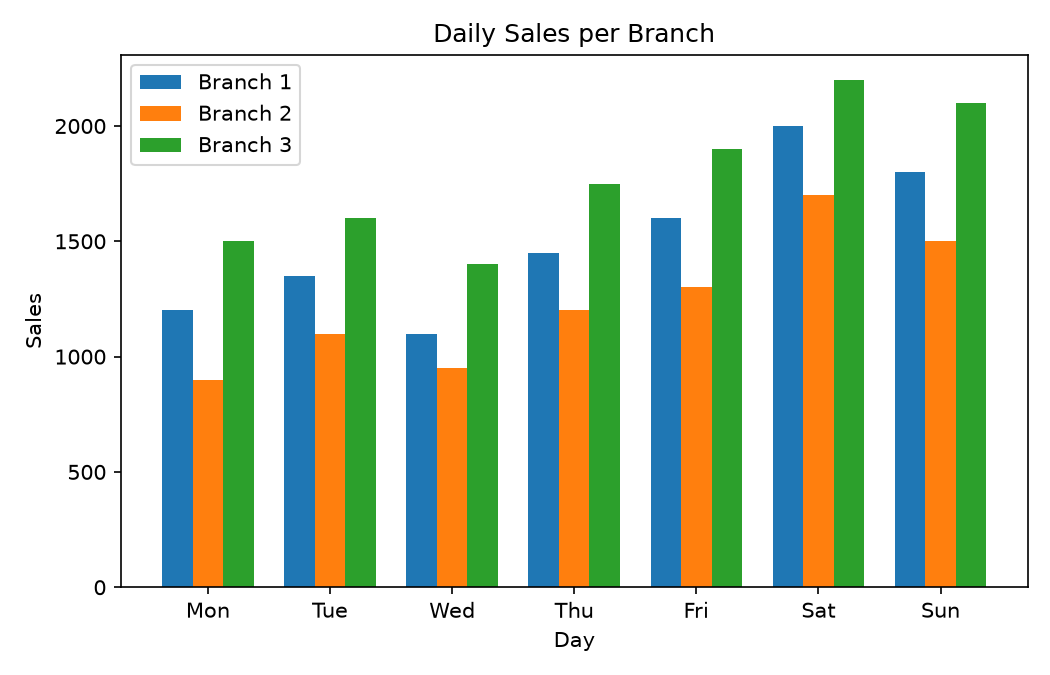
\includegraphics[width=\textwidth]{exp4_sales.png}\par{\small Fig. 1: Daily sales per branch.}\end{minipage}\hfill
\begin{minipage}{0.48\textwidth}\centering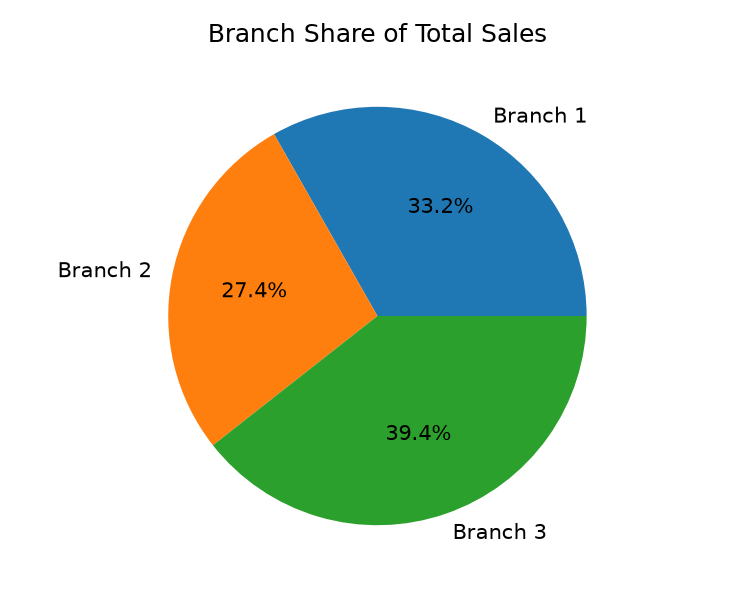
\includegraphics[width=\textwidth]{exp4_pie.png}\par{\small Fig. 2: Branch share of total sales.}\end{minipage}
\end{center}
\vspace{4pt}

\expheading{RESULT}
\vspace{4pt}
{\fontsize{12}{15}\selectfont
The above program was implemented and executed successfully using Python, and the corresponding output was obtained and verified. The results of the \textbf{NumPy data visualization} were analyzed and found to be satisfactory, thereby achieving the desired objective of the experiment.\par
}

\vspace{12pt}

\noindent\textbf{Faculty Signature:} \underline{\hspace{3.6cm}} \hfill \textbf{Date:} \underline{\hspace{2.8cm}}\par

\tooddpage

% ============================================================
% EXPERIMENT 4 : SLR hours-score (was standalone Exp 5)
% ============================================================
{\setlength{\parskip}{1pt}\setlength{\abovedisplayskip}{2pt}\setlength{\belowdisplayskip}{2pt}
\begin{center}
\expheading{EXPERIMENT NO. 3A}
\end{center}
\vspace{2pt}

\noindent\textbf{Date:} \underline{\hspace{2.6cm}} \hfill \textbf{Page No.:} \underline{\hspace{2.6cm}}\par
\vspace{6pt}

\expheading{TITLE}
\vspace{4pt}
\noindent Simple Linear Regression -- Study Hours vs Exam Score\par
\vspace{4pt}

\expheading{OBJECTIVE}
\vspace{2pt}
\fullrule
\vspace{4pt}
\noindent To implement simple linear regression on study-hours data by the regression equation and the standard (normal) equation, predict the score for 9 hours, and plot the regression line. \par
\vspace{4pt}

\expheading{AIM}
\vspace{4pt}
\noindent To fit $\hat{Y}=mX+b$ on hours-vs-score data with least squares and the normal equation, predict the 9-hour score, and evaluate with MSE and $R^2$. \par
\vspace{4pt}

\expheading{THEORY}
\vspace{4pt}
Regression equation:
\[\hat{Y}=mX+b\]
Least-squares estimates:
\[m=\frac{\sum_{i=1}^{n}(X_i-\bar{X})(Y_i-\bar{Y})}{\sum_{i=1}^{n}(X_i-\bar{X})^2}\qquad b=\bar{Y}-m\bar{X}\]
Prediction and goodness of fit:
\[\hat{Y}(9)=m\cdot9+b\qquad \mathrm{MSE}=\frac{1}{n}\sum(Y_i-\hat{Y}_i)^2\qquad R^2=1-\frac{\sum(Y_i-\hat{Y}_i)^2}{\sum(Y_i-\bar{Y})^2}\]
\vspace{4pt}

\expheading{PROCEDURE}
\vspace{4pt}
\noindent 1. Store hours (X) and scores (Y) of 8 students in NumPy arrays.\par
\noindent 2. Compute $m,b$ by least squares and by the normal equation.\par
\noindent 3. Predict the score for 9 study hours with both equations.\par
\noindent 4. Compute MSE and $R^2$; plot data points with the regression line. \par
\vspace{4pt}

\expheading{DATASET DESCRIPTION}
\vspace{4pt}
\noindent Dataset Name: Study hours vs exam score (given table)\par
\noindent Source: 8 students; X = hours (1--8), Y = score out of 100\par
\noindent Number of Samples: 8 \hspace{0.3cm} Number of Features: 1 (hours)\par
\noindent Target / Class: Exam score (0--100)\par
\noindent Description: Y = [45, 50, 54, 60, 65, 70, 74, 80]; predict at X = 9. \par
\vspace{4pt}
} % end sheet-local tightening

\toevenpage
\expheading{PROGRAM}
\vspace{6pt}

\begin{lstlisting}
import numpy as np
import matplotlib
matplotlib.use("Agg")
import matplotlib.pyplot as plt


X = np.array([1, 2, 3, 4, 5, 6, 7, 8], dtype=float)
Y = np.array([45, 50, 54, 60, 65, 70, 74, 80], dtype=float)


x_bar, y_bar = X.mean(), Y.mean()
m = ((X - x_bar) * (Y - y_bar)).sum() / ((X - x_bar) ** 2).sum()
b = y_bar - m * x_bar
print(f"Least squares: m = {m:.4f}  b = {b:.4f}")


Xb = np.c_[np.ones(len(X)), X]
t = np.linalg.inv(Xb.T @ Xb) @ Xb.T @ Y
print(f"Normal equation: b = {t[0]:.4f}  m = {t[1]:.4f}")


print(f"LS prediction for 9 hrs = {m * 9 + b:.2f}")
print(f"NE prediction for 9 hrs = {t[1] * 9 + t[0]:.2f}")


for nm, (mm, bb) in [("LS", (m, b)), ("NE", (t[1], t[0]))]:
    p = mm * X + bb
    mse = float(((Y - p) ** 2).mean())
    r2 = float(1 - ((Y - p) ** 2).sum() / ((Y - y_bar) ** 2).sum())
    print(f"{nm}: MSE={mse:.4f} R2={r2:.4f}")


plt.figure(figsize=(7, 4.5))
plt.scatter(X, Y, s=40, label="Data points")
xs = np.linspace(0, 10, 200)
plt.plot(xs, m * xs + b, linewidth=2, label="Regression line")
plt.plot(9, m * 9 + b, marker="*", markersize=14, label="Prediction (9 hrs)")
plt.xlabel("Hours study (X)")
plt.ylabel("Exam score (Y)")
plt.title("Simple Linear Regression: Study Hours vs Exam Score")
plt.legend()
plt.tight_layout()
plt.savefig("exp5_fit.png", dpi=150)
\end{lstlisting}

\tooddpage
\expheading{OUTPUT}
\vspace{2pt}
\noindent\rule{\textwidth}{0.5pt}\par
\vspace{4pt}
\begin{verbatim}
Least squares: m = 4.9762  b = 39.8571
Normal equation: b = 39.8571  m = 4.9762
LS prediction for 9 hrs = 84.64
NE prediction for 9 hrs = 84.64
LS: MSE=0.1845 R2=0.9986
NE: MSE=0.1845 R2=0.9986
\end{verbatim}
\vspace{4pt}

\begin{center}
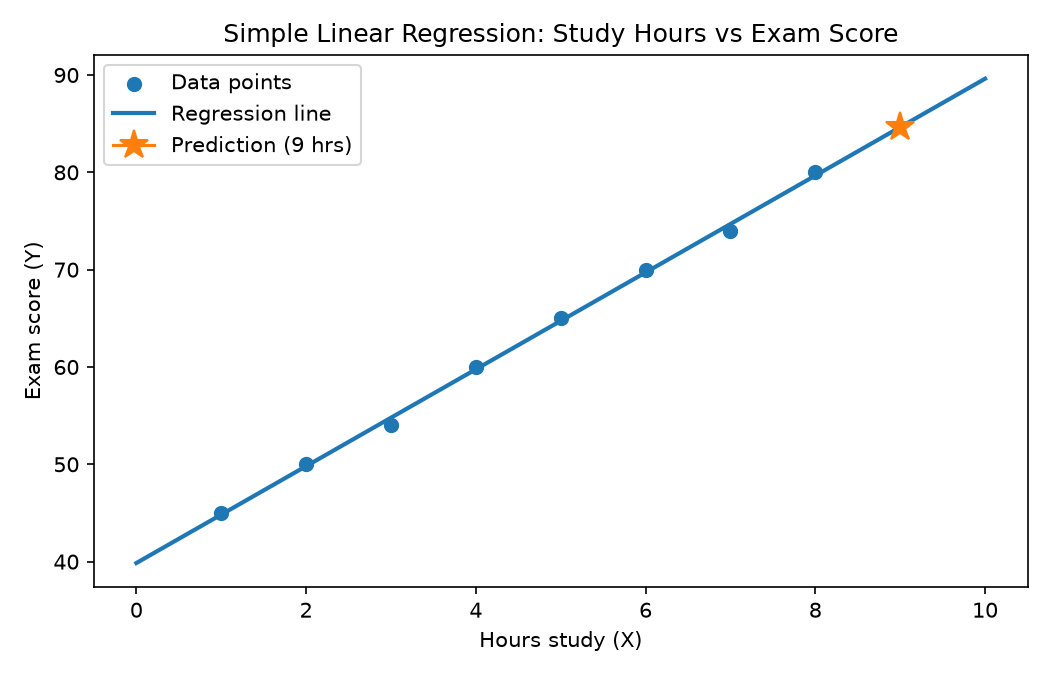
\includegraphics[width=0.78\textwidth]{exp5_fit.png}\par
\small Fig. 1: Data points, regression line and 9-hour prediction.\par
\end{center}
\vspace{4pt}

\expheading{RESULT}
\vspace{4pt}
{\fontsize{12}{15}\selectfont
The above program was implemented and executed successfully using Python, and the corresponding output was obtained and verified. The results of the \textbf{least squares regression} were analyzed and found to be satisfactory, thereby achieving the desired objective of the experiment.\par
}

\vspace{12pt}

\noindent\textbf{Faculty Signature:} \underline{\hspace{3.6cm}} \hfill \textbf{Date:} \underline{\hspace{2.8cm}}\par

\tooddpage

% ============================================================
% EXPERIMENT 5 : MLR area-age (was standalone Exp 6)
% ============================================================
{\setlength{\parskip}{1pt}\setlength{\abovedisplayskip}{2pt}\setlength{\belowdisplayskip}{2pt}
\begin{center}
\expheading{EXPERIMENT NO. 3B}
\end{center}
\vspace{2pt}

\noindent\textbf{Date:} \underline{\hspace{2.6cm}} \hfill \textbf{Page No.:} \underline{\hspace{2.6cm}}\par
\vspace{6pt}

\expheading{TITLE}
\vspace{4pt}
\noindent Multiple Linear Regression -- House Price from Area and Age\par
\vspace{4pt}

\expheading{OBJECTIVE}
\vspace{2pt}
\fullrule
\vspace{4pt}
\noindent To predict house selling price from area and age using multiple linear regression with the normal equation, and evaluate it with MSE and R-squared with a 3D plot. \par
\vspace{4pt}

\expheading{AIM}
\vspace{4pt}
\noindent To fit $\hat{Y}=b_0+b_1X_1+b_2X_2$ on the 6-house data, predict a new house price, and assess the fit. \par
\vspace{4pt}

\expheading{THEORY}
\vspace{4pt}
Regression plane (two variables):
\[\hat{Y}=b_0+b_1X_1+b_2X_2\]
Normal equation with bias column $X=[\mathbf{1}\;X_1\;X_2]$:
\[\theta=(X^TX)^{-1}X^Ty,\qquad \theta=[b_0,b_1,b_2]^T\]
Prediction and goodness of fit:
\[\hat{Y}_{new}=b_0+b_1X_{1,new}+b_2X_{2,new}\qquad \mathrm{MSE}=\frac{1}{n}\sum(Y_i-\hat{Y}_i)^2\qquad R^2=1-\frac{\sum(Y_i-\hat{Y}_i)^2}{\sum(Y_i-\bar{Y})^2}\]
\vspace{4pt}

\expheading{PROCEDURE}
\vspace{4pt}
\noindent 1. Store Area ($X_1$), Age ($X_2$) and Price ($Y$) of 6 houses in NumPy arrays.\par
\noindent 2. Build $X$ with a bias column and solve $\theta=(X^TX)^{-1}X^Ty$.\par
\noindent 3. Predict the price of a new house (Area 2.8, Age 4).\par
\noindent 4. Compute MSE and $R^2$; plot houses with the fitted plane in 3D. \par
\vspace{4pt}

\expheading{DATASET DESCRIPTION}
\vspace{4pt}
\noindent Dataset Name: House price vs area and age (given table)\par
\noindent Source: 6 houses; $X_1$ = area, $X_2$ = age (years), $Y$ = price (lakhs)\par
\noindent Number of Samples: 6 \hspace{0.3cm} Number of Features: 2\par
\noindent Target / Class: Selling price in lakhs\par
\noindent Description: Area=[1.0--3.5]; Age=[10--2]; Price=[20--43]. \par
\vspace{4pt}
} % end sheet-local tightening

\toevenpage
\expheading{PROGRAM}
\vspace{6pt}

\begin{lstlisting}
import numpy as np
import matplotlib
matplotlib.use("Agg")
import matplotlib.pyplot as plt


X1 = np.array([1.0, 1.5, 2.0, 2.5, 3.0, 3.5])
X2 = np.array([10, 8, 6, 5, 3, 2], dtype=float)
Y = np.array([20, 24, 29, 32, 38, 43], dtype=float)


Xb = np.c_[np.ones(len(X1)), X1, X2]
t = np.linalg.inv(Xb.T @ Xb) @ Xb.T @ Y
b0, b1, b2 = t
print(f"Plane: Y = {b0:.4f} + {b1:.4f}*Area + {b2:.4f}*Age")


p = Xb @ t
mse = float(((Y - p) ** 2).mean())
r2 = float(1 - ((Y - p) ** 2).sum() / ((Y - Y.mean()) ** 2).sum())
print(f"MLR: MSE={mse:.4f} R2={r2:.4f} RMSE={np.sqrt(mse):.4f}")


new = b0 + b1 * 2.8 + b2 * 4
print(f"Predicted price (Area 2.8, Age 4) = {new:.2f} lakhs")


fig = plt.figure(figsize=(7, 5))
ax = fig.add_subplot(111, projection="3d")
ax.scatter(X1, X2, Y, s=40, label="Houses")
a = np.linspace(0.8, 3.7, 20)
g = np.linspace(1, 11, 20)
A, G = np.meshgrid(a, g)
ax.plot_surface(A, G, b0 + b1 * A + b2 * G, alpha=0.4)
ax.scatter([2.8], [4], [new], s=80, marker="*",
           label="Prediction (2.8, 4)")
ax.set_xlabel("Area X1")
ax.set_ylabel("Age X2")
ax.set_zlabel("Price Y (lakhs)")
ax.set_title("Multiple Linear Regression: Price vs Area and Age")
ax.legend()
plt.tight_layout()
plt.savefig("exp6_plane.png", dpi=150)
\end{lstlisting}

\tooddpage
\expheading{OUTPUT}
\vspace{2pt}
\noindent\rule{\textwidth}{0.5pt}\par
\vspace{4pt}
\begin{verbatim}
Plane: Y = 10.4286 + 9.1429*Area + 0.0000*Age
MLR: MSE=0.3810 R2=0.9938 RMSE=0.6172
Predicted price (Area 2.8, Age 4) = 36.03 lakhs
\end{verbatim}
\vspace{4pt}

\begin{center}
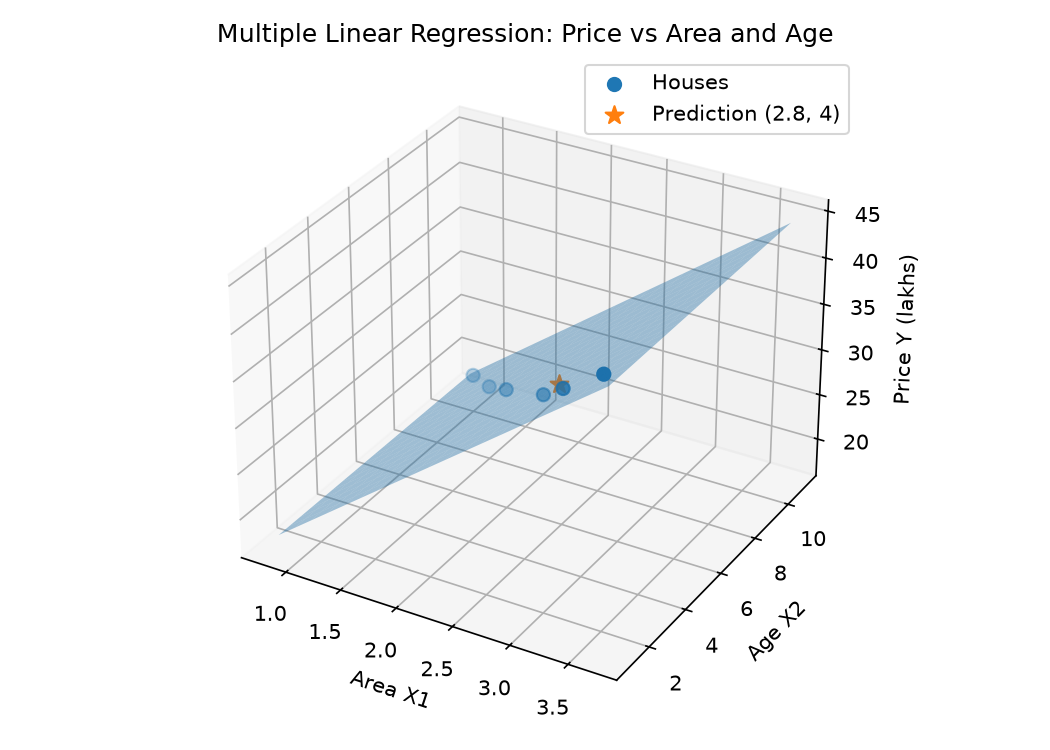
\includegraphics[width=0.78\textwidth]{exp6_plane.png}\par
\small Fig. 1: Houses, fitted plane and predicted house (star).\par
\end{center}
\vspace{4pt}

\expheading{RESULT}
\vspace{4pt}
{\fontsize{12}{15}\selectfont
The above program was implemented and executed successfully using Python, and the corresponding output was obtained and verified. The results of the \textbf{multiple linear regression} were analyzed and found to be satisfactory, thereby achieving the desired objective of the experiment.\par
}

\vspace{12pt}

\noindent\textbf{Faculty Signature:} \underline{\hspace{3.6cm}} \hfill \textbf{Date:} \underline{\hspace{2.8cm}}\par

\tooddpage

% ============================================================
% EXPERIMENT 4A
% ============================================================
{\setlength{\parskip}{1pt}\setlength{\abovedisplayskip}{2pt}\setlength{\belowdisplayskip}{2pt}
\begin{center}
\expheading{EXPERIMENT NO. 4A}
\end{center}
\vspace{2pt}

\noindent\textbf{Date:} \underline{\hspace{2.6cm}} \hfill \textbf{Page No.:} \underline{\hspace{2.6cm}}\par
\vspace{6pt}

\expheading{TITLE}
\vspace{4pt}
\noindent Simple Linear Regression using Least Squares -- TotalRooms\par
\vspace{4pt}

\expheading{OBJECTIVE}
\vspace{2pt}
\fullrule
\vspace{4pt}
\noindent To implement least squares regression on housing.csv (X=TotalRooms, Y=MedHouseVal) and evaluate it with MSE, R-squared and the regression-line plot. \par
\vspace{4pt}

\expheading{AIM}
\vspace{4pt}
\noindent To fit $\hat{Y}=mX+b$ by least squares on TotalRooms, predict test values, and assess the fit with MSE and $R^2$. \par
\vspace{4pt}

\expheading{THEORY}
\vspace{4pt}
Regression equation:
\[\hat{Y}=mX+b\]
Least-squares estimates:
\[m=\frac{\sum_{i=1}^{n}(X_i-\bar{X})(Y_i-\bar{Y})}{\sum_{i=1}^{n}(X_i-\bar{X})^2}\qquad b=\bar{Y}-m\bar{X}\]
Goodness of fit:
\[\mathrm{MSE}=\frac{1}{n}\sum_{i=1}^{n}(Y_i-\hat{Y}_i)^2\qquad R^2=1-\frac{\sum_{i=1}^{n}(Y_i-\hat{Y}_i)^2}{\sum_{i=1}^{n}(Y_i-\bar{Y})^2}\]
\vspace{4pt}

\expheading{PROCEDURE}
\vspace{4pt}
\noindent B) Load the California Housing dataset (housing.csv).\par
\noindent C) Identify the variables: independent $X=$ TotalRooms (Total rooms); dependent $Y=$ MedHouseVal (Median House Value).\par
\noindent D) Inspect the dataset for missing, duplicate, or invalid values.\par
\noindent E) Calculate the slope $m$ and the intercept $b$ using the least square equation.\par
\noindent F) Construct the regression equation $\hat{Y}=mX+b$.\par
\noindent G) Use the regression equation to predict the target values for the test dataset.\par
\noindent H) Calculate the Mean Squared Error (MSE) and the coefficient of determination $R^2$ to measure the goodness of fit.\par
\noindent I) Plot the actual data points and regression line. \par
\vspace{4pt}

\expheading{DATASET DESCRIPTION}
\vspace{4pt}
\noindent Dataset Name: California Housing (housing.csv)\par
\noindent Source: Public census CSV file; prepared with NumPy only\par
\noindent Number of Samples: 20640 usable (0 missing) \hspace{0.3cm} Number of Features: 1 (TotalRooms)\par
\noindent Target / Class: MedHouseVal $-$ median house value in units of \$100{,}000\par
\noindent Description: Train 16512 / test 4128 (80/20, seed 42). \par
\vspace{4pt}
} % end sheet-local tightening
\toevenpage
\expheading{PROGRAM}
\vspace{6pt}

\begin{lstlisting}
import csv
import numpy as np
import matplotlib
matplotlib.use("Agg")
import matplotlib.pyplot as plt
rooms, prices, miss = [], [], 0
with open("housing.csv", newline="") as f:
    for r in csv.DictReader(f):
        try:
            rooms.append(float(r["total_rooms"]))
            prices.append(float(r["median_house_value"]))
        except (ValueError, KeyError):
            miss += 1
X = np.array(rooms)
y = np.array(prices) / 1e5
print("Usable:", len(X), " Missing:", miss)
rng = np.random.default_rng(42)
order = np.arange(len(X))
rng.shuffle(order)
n_train = int(0.8 * len(X))
X_train, X_test = X[order[:n_train]], X[order[n_train:]]
y_train, y_test = y[order[:n_train]], y[order[n_train:]]
print("Train:", len(X_train), " Test:", len(X_test))
x_bar = X_train.mean()
y_bar = y_train.mean()
m = ((X_train - x_bar) * (y_train - y_bar)).sum()
m = m / ((X_train - x_bar) ** 2).sum()
b = y_bar - m * x_bar
print(f"LS slope m = {m:.6f}")
print(f"LS intercept b = {b:.4f}")
y_pred = m * X_test + b
mse = ((y_test - y_pred) ** 2).mean()
r2 = 1 - ((y_test - y_pred) ** 2).sum() / ((y_test - y_test.mean()) ** 2).sum()
print(f"LS: MSE={mse:.4f} R2={r2:.4f} RMSE={np.sqrt(mse):.4f}")
plt.figure(figsize=(7, 4.5))
plt.scatter(X_test, y_test, s=6, alpha=0.25, label="Test data")
xs = np.linspace(0, float(np.percentile(X, 99.5)), 200)
plt.plot(xs, m * xs + b, linewidth=2, label="Least Squares line")
plt.xlabel("TotalRooms (X)")
plt.ylabel("MedHouseVal ($100k) (Y)")
plt.title("Simple Linear Regression (Least Squares): TotalRooms vs Price")
plt.legend()
plt.tight_layout()
plt.savefig("exp4a_fit.png", dpi=150)
\end{lstlisting}
\tooddpage
\expheading{OUTPUT}
\vspace{2pt}
\noindent\rule{\textwidth}{0.5pt}\par
\vspace{4pt}
\begin{verbatim}
Usable: 20640  Missing: 0
Train: 16512  Test: 4128
LS slope m = 0.000072
LS intercept b = 1.8840
LS: MSE=1.3236 R2=0.0167 RMSE=1.1505
\end{verbatim}
\vspace{4pt}

\begin{center}
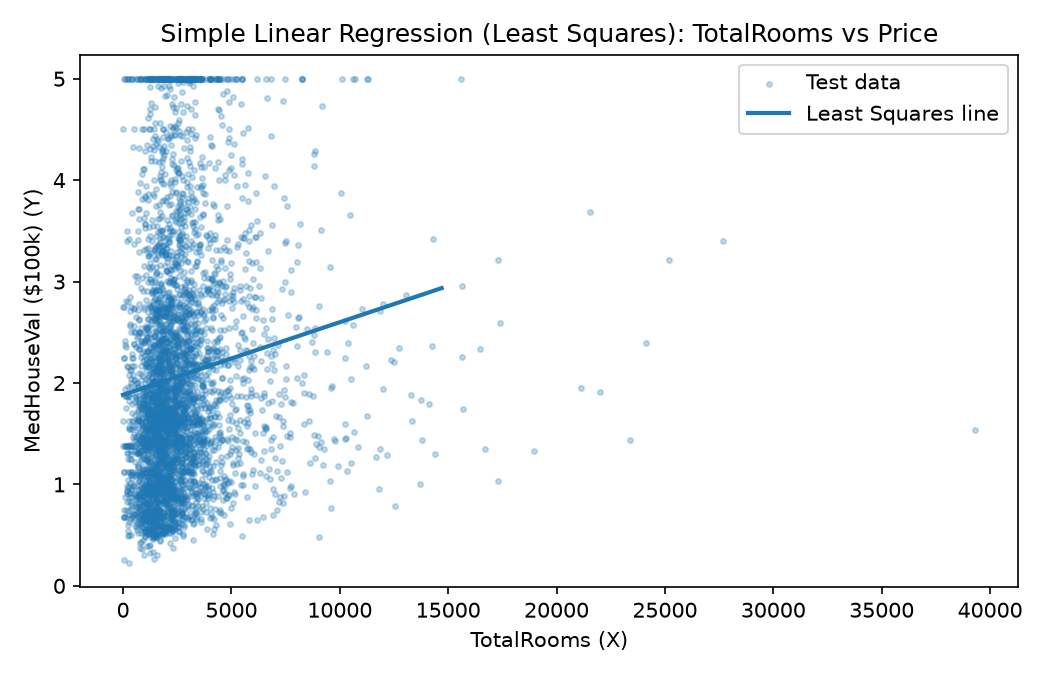
\includegraphics[width=0.78\textwidth]{exp4a_fit.png}\par
\small Fig. 1: Test data with the least-squares regression line.\par
\end{center}
\vspace{4pt}

\expheading{RESULT}
\vspace{4pt}
{\fontsize{12}{15}\selectfont
The above program was implemented and executed successfully using Python, and the corresponding output was obtained and verified. The results of the \textbf{least squares regression} were analyzed and found to be satisfactory, thereby achieving the desired objective of the experiment.\par
}

\vspace{12pt}

\noindent\textbf{Faculty Signature:} \underline{\hspace{3.6cm}} \hfill \textbf{Date:} \underline{\hspace{2.8cm}}\par

\tooddpage

% ============================================================
% EXPERIMENT 4B
% ============================================================
{\setlength{\parskip}{1pt}\setlength{\abovedisplayskip}{2pt}\setlength{\belowdisplayskip}{2pt}
\begin{center}
\expheading{EXPERIMENT NO. 4B}
\end{center}
\vspace{2pt}

\noindent\textbf{Date:} \underline{\hspace{2.6cm}} \hfill \textbf{Page No.:} \underline{\hspace{2.6cm}}\par
\vspace{6pt}

\expheading{TITLE}
\vspace{4pt}
\noindent Simple Linear Regression using Gradient Descent -- TotalRooms\par
\vspace{4pt}

\expheading{OBJECTIVE}
\vspace{2pt}
\fullrule
\vspace{4pt}
\noindent To implement gradient descent regression on housing.csv (X=TotalRooms, Y=MedHouseVal) with $\alpha=0.01$ and 100 epochs, and evaluate it with MSE, R-squared and the cost curve. \par
\vspace{4pt}

\expheading{AIM}
\vspace{4pt}
\noindent To fit $\hat{Y}=mX+b$ by gradient descent from $m=c=0$, predict test values, and assess with MSE and $R^2$. \par
\vspace{4pt}

\expheading{THEORY}
\vspace{4pt}
Linear hypothesis:
\[\hat{Y}=mX+b\]
Mean Squared Error cost:
\[J(m,c)=\frac{1}{n}\sum_{i=1}^{n}(Y_i-\hat{Y}_i)^2\]
Gradients:
\[\frac{\partial J}{\partial m}=-\frac{2}{n}\sum_{i=1}^{n}X_i(Y_i-\hat{Y}_i)\qquad \frac{\partial J}{\partial b}=-\frac{2}{n}\sum_{i=1}^{n}(Y_i-\hat{Y}_i)\]
Gradient descent updates:
\[m:=m-\alpha\frac{\partial J}{\partial m}\qquad b:=b-\alpha\frac{\partial J}{\partial b}\]
\vspace{4pt}

\expheading{PROCEDURE}
\vspace{4pt}
\noindent 1. Load the California Housing dataset and select TotalRooms as $X$ and MedHouseVal as $Y$.\par
\noindent 2. Inspect and clean the data by checking missing and invalid values.\par
\noindent 3. Split the dataset into training and testing sets.\par
\noindent 4. Standardize the input feature using the mean and standard deviation of the training data.\par
\noindent 5. Initialize slope $m=0$ and intercept $c=0$.\par
\noindent 6. Choose learning rate $\alpha=0.01$ and epochs $=100$.\par
\noindent 7. Calculate the predicted values.\par
\noindent 8. Calculate the Mean Squared Error cost $J(m,c)=\frac{1}{n}\sum(Y_i-\hat{Y}_i)^2$.\par
\noindent 9. Calculate the gradient w.r.t.\ slope $\frac{\partial J}{\partial m}=-\frac{2}{n}\sum X_i(Y_i-\hat{Y}_i)$.\par
\noindent 10. Calculate the gradient w.r.t.\ intercept $\frac{\partial J}{\partial b}=-\frac{2}{n}\sum(Y_i-\hat{Y}_i)$.\par
\noindent 11. Update slope $m=m-\alpha\frac{\partial J}{\partial m}$ and intercept $b=b-\alpha\frac{\partial J}{\partial b}$.\par
\noindent 12. Repeat steps 8--11 for 100 epochs or until the cost converges.\par
\noindent 13. Plot cost versus epochs to verify convergence.\par
\noindent 14. Predict test values with final $m,b$; calculate MSE and $R^2$. \par
\vspace{4pt}

\expheading{DATASET DESCRIPTION}
\vspace{4pt}
\noindent Dataset Name: California Housing (housing.csv)\par
\noindent Source: Public census CSV file; prepared with NumPy only; feature standardized\par
\noindent Number of Samples: 20640 usable (0 missing) \hspace{0.3cm} Number of Features: 1 (TotalRooms)\par
\noindent Target / Class: MedHouseVal $-$ median house value in units of \$100{,}000\par
\noindent Description: Train 16512 / test 4128 (80/20, seed 42). \par
\vspace{4pt}
} % end sheet-local tightening
\toevenpage
\expheading{PROGRAM}
\vspace{6pt}

\begin{lstlisting}
import csv
import numpy as np
import matplotlib
matplotlib.use("Agg")
import matplotlib.pyplot as plt
rooms, prices, miss = [], [], 0
with open("housing.csv", newline="") as f:
    for r in csv.DictReader(f):
        try:
            rooms.append(float(r["total_rooms"]))
            prices.append(float(r["median_house_value"]))
        except (ValueError, KeyError):
            miss += 1
X = np.array(rooms)
y = np.array(prices) / 1e5
print("Usable:", len(X), " Missing:", miss)
rng = np.random.default_rng(42)
order = np.arange(len(X))
rng.shuffle(order)
n_train = int(0.8 * len(X))
X_train, X_test = X[order[:n_train]], X[order[n_train:]]
y_train, y_test = y[order[:n_train]], y[order[n_train:]]
print("Train:", len(X_train), " Test:", len(X_test))
mu = X_train.mean()
sg = X_train.std()
Xs_train = (X_train - mu) / sg
m, b = 0.0, 0.0
n = len(Xs_train)
costs = []
for epoch in range(100):
    y_hat = m * Xs_train + b
    err = y_train - y_hat
    J = (err ** 2).mean()
    costs.append(float(J))
    dm = (-2 / n) * (Xs_train * err).sum()
    db = (-2 / n) * err.sum()
    m = m - 0.01 * dm
    b = b - 0.01 * db
m_gd = m / sg
b_gd = b - m * mu / sg
print(f"GD slope m = {m_gd:.6f}")
print(f"GD intercept b = {b_gd:.4f}")
print(f"GD cost first={costs[0]:.4f} last={costs[-1]:.4f}")
y_pred = m_gd * X_test + b_gd
mse = ((y_test - y_pred) ** 2).mean()
r2 = 1 - ((y_test - y_pred) ** 2).sum() / ((y_test - y_test.mean()) ** 2).sum()
print(f"GD: MSE={mse:.4f} R2={r2:.4f} RMSE={np.sqrt(mse):.4f}")
plt.figure(figsize=(6, 3.8))
plt.plot(range(1, 101), costs)
plt.xlabel("Epoch")
plt.ylabel("Cost J (MSE)")
plt.title("Gradient Descent: Cost vs Epochs")
plt.tight_layout()
plt.savefig("exp4b_cost.png", dpi=150)
\end{lstlisting}
\tooddpage
\expheading{OUTPUT}
\vspace{2pt}
\noindent\rule{\textwidth}{0.5pt}\par
\vspace{4pt}
\begin{verbatim}
Usable: 20640  Missing: 0
Train: 16512  Test: 4128
GD slope m = 0.000062
GD intercept b = 1.6341
GD cost first=5.6208 last=1.3827
GD: MSE=1.3885 R2=-0.0315 RMSE=1.1784
\end{verbatim}
\vspace{4pt}

\begin{center}
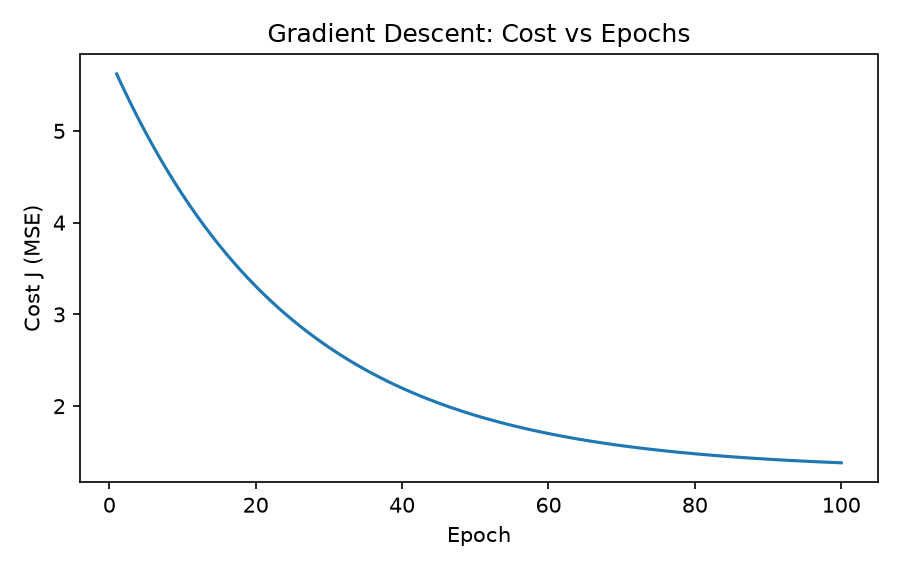
\includegraphics[width=0.62\textwidth]{exp4b_cost.png}\par
\small Fig. 2: Gradient-descent cost vs epochs ($\alpha=0.01$, 100 epochs).\par
\end{center}
\vspace{4pt}

\expheading{RESULT}
\vspace{4pt}
{\fontsize{12}{15}\selectfont
The above program was implemented and executed successfully using Python, and the corresponding output was obtained and verified. The results of the \textbf{gradient descent regression} were analyzed and found to be satisfactory, thereby achieving the desired objective of the experiment.\par
}

\vspace{12pt}

\noindent\textbf{Faculty Signature:} \underline{\hspace{3.6cm}} \hfill \textbf{Date:} \underline{\hspace{2.8cm}}\par

\tooddpage

% ============================================================
% EXPERIMENT 4C
% ============================================================
{\setlength{\parskip}{1pt}\setlength{\abovedisplayskip}{2pt}\setlength{\belowdisplayskip}{2pt}
\begin{center}
\expheading{EXPERIMENT NO. 4C}
\end{center}
\vspace{2pt}

\noindent\textbf{Date:} \underline{\hspace{2.6cm}} \hfill \textbf{Page No.:} \underline{\hspace{2.6cm}}\par
\vspace{6pt}

\expheading{TITLE}
\vspace{4pt}
\noindent Simple Linear Regression with Scikit-learn -- AveRooms\par
\vspace{4pt}

\expheading{OBJECTIVE}
\vspace{2pt}
\fullrule
\vspace{4pt}
\noindent To implement simple linear regression with Scikit-learn on the California Housing dataset (X=AveRooms, Y=MedHouseVal) and evaluate it with MSE, R-squared and the regression-line plot. \par
\vspace{4pt}

\expheading{AIM}
\vspace{4pt}
\noindent To fit the sklearn LinearRegression model on AveRooms, predict test values, and assess with MSE and $R^2$. \par
\vspace{4pt}

\expheading{THEORY}
\vspace{4pt}
Linear hypothesis:
\[\hat{Y}=mX+b\]
Scikit-learn fits $m,b$ by least squares (normal equation via SVD).
Goodness of fit:
\[\mathrm{MSE}=\frac{1}{n}\sum_{i=1}^{n}(Y_i-\hat{Y}_i)^2\qquad R^2=1-\frac{\sum_{i=1}^{n}(Y_i-\hat{Y}_i)^2}{\sum_{i=1}^{n}(Y_i-\bar{Y})^2}\]
\vspace{4pt}

\expheading{PROCEDURE}
\vspace{4pt}
\noindent 1. Import NumPy and Pandas for data handling; fetch\_california\_housing, train\_test\_split, LinearRegression, mean\_squared\_error, r2\_score and Matplotlib.\par
\noindent 2. Load with fetch\_california\_housing(); build the DataFrame; assign feature names; separate the target.\par
\noindent 3. Explore: first records, shape, features and missing values.\par
\noindent 4. Take X=AveRooms, Y=MedHouseVal; scatter AveRooms vs MedHouseVal.\par
\noindent 5. Split 80/20 (random\_state=42); fit LinearRegression; read slope $m$ and intercept $b$.\par
\noindent 6. Predict test values; report MSE and $R^2$; plot test points with the regression line, labels, title and legend. \par
\vspace{4pt}

\expheading{DATASET DESCRIPTION}
\vspace{4pt}
\noindent Dataset Name: California Housing via Scikit-learn\par
\noindent Source: fetch\_california\_housing (1990 census)\par
\noindent Number of Samples: 20640 \hspace{0.3cm} Number of Features: 8 (X=AveRooms)\par
\noindent Target / Class: MedHouseVal $-$ median house value in units of \$100{,}000\par
\noindent Description: Train 16512 / test 4128 (80/20, random\_state=42). \par
\vspace{4pt}
} % end sheet-local tightening
\toevenpage
\expheading{PROGRAM}
\vspace{6pt}

\begin{lstlisting}
import numpy as np
import pandas as pd
import matplotlib
matplotlib.use("Agg")
import matplotlib.pyplot as plt
from sklearn.datasets import fetch_california_housing
from sklearn.model_selection import train_test_split
from sklearn.linear_model import LinearRegression
from sklearn.metrics import mean_squared_error, r2_score
housing = fetch_california_housing()
df = pd.DataFrame(housing.data, columns=housing.feature_names)
print("Shape:", df.shape)
print("Missing:", int(df.isnull().sum().sum()))
X = df[["AveRooms"]]
y = housing.target
X_train, X_test, y_train, y_test = train_test_split(
    X, y, test_size=0.2, random_state=42)
print("Train:", len(X_train), " Test:", len(X_test))
model = LinearRegression()
model.fit(X_train, y_train)
print(f"m = {model.coef_[0]:.6f} b = {model.intercept_:.4f}")
p = model.predict(X_test)
print(f"MSE={mean_squared_error(y_test, p):.4f} "
      f"R2={r2_score(y_test, p):.4f} RMSE={np.sqrt(mean_squared_error(y_test, p)):.4f}")
plt.figure(figsize=(7, 4.5))
plt.scatter(X_test, y_test, s=6, alpha=0.25, label="Test data")
xs = np.linspace(0, 15, 200)
plt.plot(xs, model.coef_[0] * xs + model.intercept_,
         linewidth=2, label="Sklearn line")
plt.xlim(0, 15)
plt.xlabel("AveRooms")
plt.ylabel("MedHouseVal ($100k)")
plt.title("Simple Linear Regression with Scikit-learn")
plt.legend()
plt.tight_layout()
plt.savefig("exp4c_fit.png", dpi=150)
\end{lstlisting}
\tooddpage
\expheading{OUTPUT}
\vspace{2pt}
\noindent\rule{\textwidth}{0.5pt}\par
\vspace{4pt}
\begin{verbatim}
Shape: (20640, 8)
Missing: 0
Train: 16512  Test: 4128
m = 0.076756 b = 1.6548
MSE=1.2923 R2=0.0138 RMSE=1.1368
\end{verbatim}
\vspace{4pt}

\begin{center}
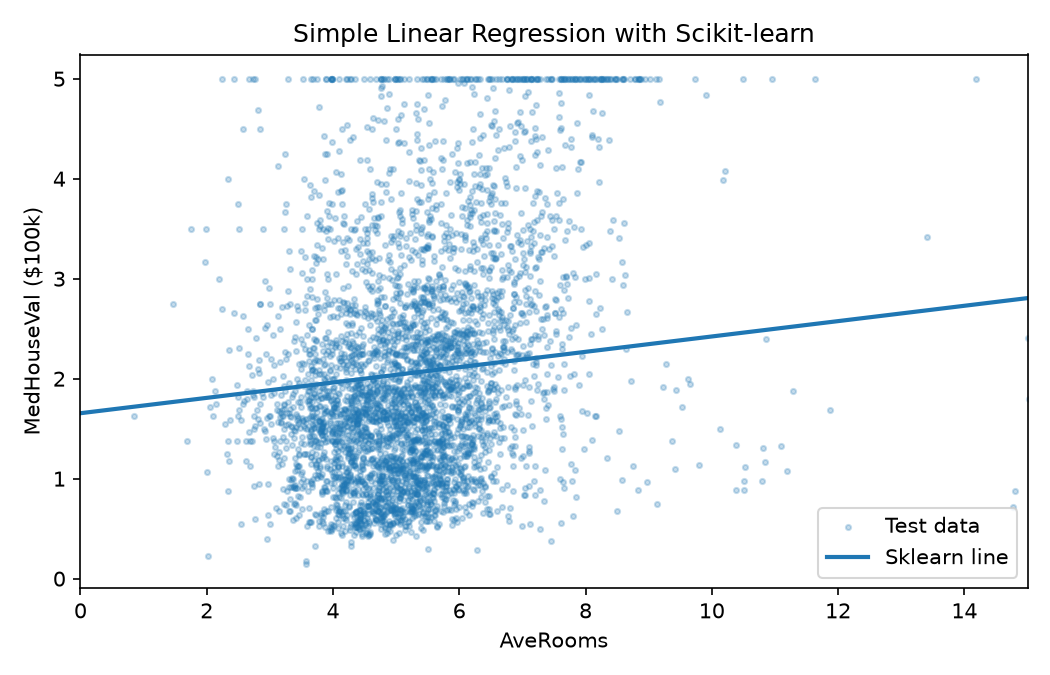
\includegraphics[width=0.78\textwidth]{exp4c_fit.png}\par
\small Fig. 1: Test data with the Scikit-learn regression line.\par
\end{center}
\vspace{4pt}

\expheading{RESULT}
\vspace{4pt}
{\fontsize{12}{15}\selectfont
The above program was implemented and executed successfully using Python, and the corresponding output was obtained and verified. The results of the \textbf{Scikit-learn LinearRegression model} were analyzed and found to be satisfactory, thereby achieving the desired objective of the experiment.\par
}

\vspace{12pt}

\noindent\textbf{Faculty Signature:} \underline{\hspace{3.6cm}} \hfill \textbf{Date:} \underline{\hspace{2.8cm}}\par

\end{document}
